\documentclass{beamer}
\usepackage{amsmath}
\usepackage{graphicx}
\usepackage{tikz}
\usetikzlibrary{tikzmark, decorations.pathreplacing}
\setbeamertemplate{caption}[numbered]
\setbeamerfont{caption}{size=\scriptsize}
\setbeamertemplate{navigation symbols}{} %remove navigation symbols
\usepackage[style=apa, backend=biber]{biblatex}
%\setbeamertemplate{bibliography item}{}
%\addbibresource{library.bib}

%\usetheme{default}
%\usetheme{AnnArbor}
%\usetheme{Antibes}
%\usetheme{Bergen}
%\usetheme{Berkeley}
%\usetheme{Berlin}
%\usetheme{Boadilla}
%\usetheme{CambridgeUS}
%\usetheme{Copenhagen}
%\usetheme{Darmstadt}
\usetheme{Dresden}
%\usetheme{Frankfurt}
%\usetheme{Goettingen}
%\usetheme{Hannover}
%\usetheme{Ilmenau}
%\usetheme{JuanLesPins}
%\usetheme{Luebeck}
%\usetheme{Madrid}
%\usetheme{Malmoe}
%\usetheme{Marburg}
%\usetheme{Montpellier}
%\usetheme{PaloAlto}
%\usetheme{Pittsburgh}
%\usetheme{Rochester}
%\usetheme{Singapore}
%\usetheme{Szeged}
%\usetheme{Warsaw}

% \usepackage{beamerthemesplit} // Activate for custom appearance
%\usecolortheme{albatross}
%\usecolortheme{beaver}
%\usecolortheme{beetle}
%\usecolortheme{crane}
%\usecolortheme{dolphin}%cok guzel bu
%\usecolortheme{dove}
%\usecolortheme{fly}
%\usecolortheme{lily}
%\usecolortheme{orchid}
%\usecolortheme{rose}
%\usecolortheme{seagull}
%\usecolortheme{seahorse}
\usecolortheme{whale}
%\usecolortheme{wolverine}
%\setbeamertemplate{footline} % To remove the footer line in all slides uncomment this line
\setbeamertemplate{footline}[page number] % To replace the footer line in all slides with a simple slide count uncomment this line

\title{Does armed conflict influence population size?}
\subtitle{For presentation at PHAC workshop, Illinois, October 2023}

\author{Wesley Wang, MPhil Student, University of Oxford \\
Nathalie Williams, Professor, University of Washington}
\date{\ }

\begin{document}
	\begin{frame}
		\titlepage	
	\end{frame}
	
	\section{Overview}

		\begin{frame}{Agenda}
			\tableofcontents 
		\end{frame}

	\section{Research Question}
		\begin{frame}{Research Question \& Significance}
			\textbf{How does armed conflict influence population size?}
				\begin{itemize}
					\item More people or fewer people?
					\begin{itemize}
						\item Short term
						\item Long term
					\end{itemize}
				\end{itemize}

			\textbf{Why is this important?}
				\begin{itemize}
					\item Armed conflict common globally
					\item Policy making
					\item Population projection
					\item Shocks that are pervasive beyond armed conflict
				\end{itemize}
		\end{frame}

		\begin{frame}{Don't we know this? People die!}
			\textbf{Armed conflict:}
				\begin{itemize}
					\item People die \tikzmark{start1}
					\item People get sick/injured \tikzmark{end1}
				\end{itemize}

				\begin{tikzpicture}[remember picture,overlay]
					\draw[decorate,decoration={brace,raise=12pt}]
					  ([yshift=2ex]{{pic cs:end1}|-{pic cs:start1}}) --
						node[xshift=15pt,anchor=west] {Fewer people} 
					  ([yshift=-0.5ex]pic cs:end1);
					\end{tikzpicture}

			\textbf{Armed conflict X other demographic behaviours:}
				\begin{itemize}
					\item Marriage rates \tikzmark{start}
					\item Age at marriage
					\item Fertility rates
					\item Age at births
					\item Education
					\item Employment
					\item Etc. \tikzmark{end}
				\end{itemize}

				\begin{tikzpicture}[remember picture,overlay]
					\draw[decorate,decoration={brace,raise=59pt}]
					  ([yshift=2ex]{{pic cs:end}|-{pic cs:start}}) --
						node[xshift=66pt,anchor=west] {Fewer people?  We have no idea!} 
					  ([yshift=-0.5ex]pic cs:end);
					\end{tikzpicture}
		\end{frame}

	\section{Conceptual Framework}
		\begin{frame}{Conceptual Framework}
			%\begin{columns}
			%	\begin{column}{0.5\textwidth}
			%	  \includegraphics[width=\linewidth]{Images/linear1.png}
			%	\end{column}
			%	\begin{column}{0.5\textwidth}
			%		\includegraphics[width=\linewidth]{Images/linear2.png}
			%	\end{column}
			% \end{columns}
			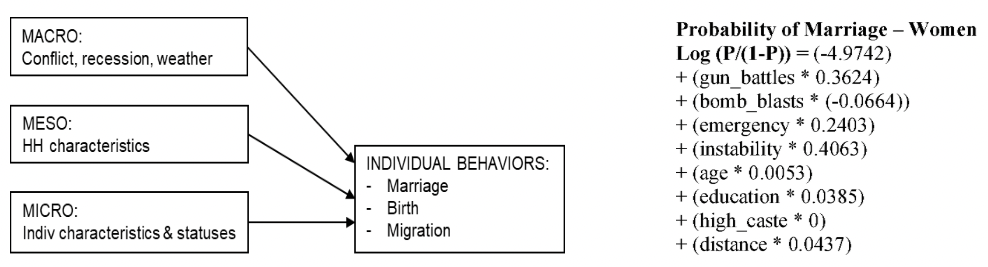
\includegraphics[width=\linewidth]{Images/con1.png}
		\end{frame}

		\begin{frame}{Conceptual Framework}
			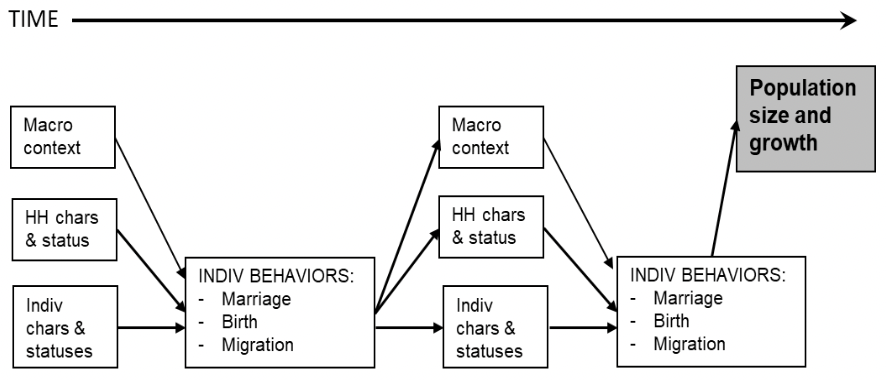
\includegraphics[width=\linewidth]{Images/con2.png}
		\end{frame}

	\section{Methods}

		\begin{frame}{Agent-based Models}
			\textbf{Computational simulation of hypothetical population}
			\begin{itemize}
				\item Agents
			\end{itemize}
		\end{frame}


		\begin{frame}{Agent-based Models}
			\textbf{Computational simulation of hypothetical population}
			\begin{itemize}
				\item Agents
				\item Behavioural rules
			\end{itemize}
			
			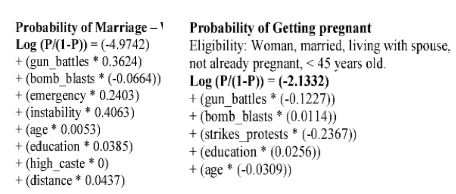
\includegraphics[width=0.8\textwidth]{Images/method1.png}
		\end{frame}

		\begin{frame}{Agent-based Models}
			\textbf{Computational simulation of hypothetical population}
			\begin{itemize}
				\item Agents
				\item Behavioural rules
				\item Simulate war
			\end{itemize}

			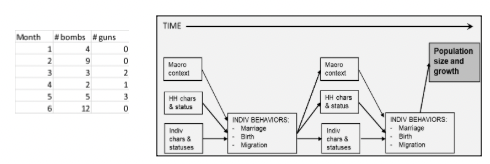
\includegraphics[width=0.9\textwidth]{Images/method2.png}
		\end{frame}
		
		\begin{frame}{Agent-based Models}
			\textbf{What do you get out of this?}
			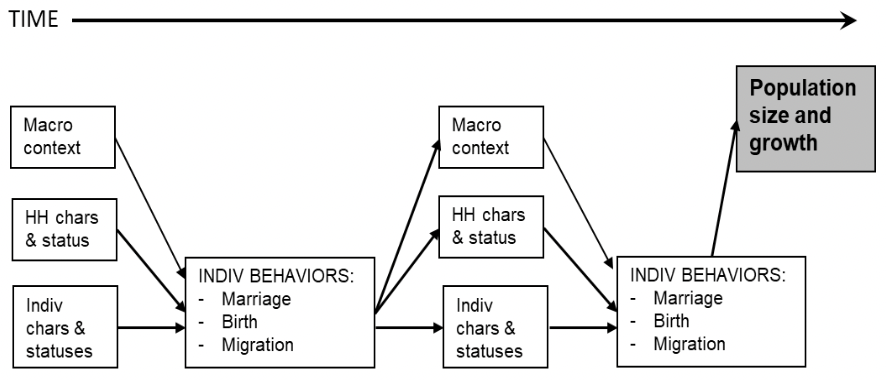
\includegraphics[width=0.7\textwidth]{Images/con2.png}

			\begin{itemize}
				\item Complex, non-linear population dynamics
				\item Interactions with time-varying context (war)
				\item Micro-level behaviours to macro-level outcomes
			\end{itemize}

		\end{frame}

		\begin{frame}{Agent-based Models}
			\textbf{What do you get out of this?}
			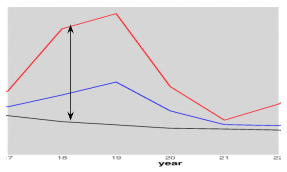
\includegraphics[width=0.7\textwidth]{Images/method3.png}

			\begin{itemize}
				\item Experimental laboratory
					\begin{itemize}
						\item Number of people in war scenario?
						\item Number people in non-war scenario?
					\end{itemize}
			\end{itemize}
		\end{frame}

	\section{Setting}
		\begin{frame}{Our ABM}
			\textbf{Chitwan Valley}
			
			\begin{itemize}
				\item Rural agricultural area
				\item 5 year armed conflict 
				\item ABM population matches real population -- survey data (CVFS)
				\item Behavioural rules: Regression equations from survey data (CVFS)
				\item Armed conflict events: INSEC, SATP, local sources, news 
			\end{itemize}
		\end{frame}

	\section{Results}
		\begin{frame}{Population Size}
			\begin{center}
				\begin{figure}
					\includegraphics[width=\textwidth]{Images/popsize.png}
					\caption{Population size (Conflict period)}
				\end{figure}
			\end{center} 	

			\begin{itemize}
				\item LARGER population during and after conflict period
			\end{itemize}
		\end{frame}

		\begin{frame}{Population Growth}
			\begin{center}
				\begin{figure}
					\includegraphics[width=\textwidth]{Images/popgrowth.png}
					\caption{Population growth (Conflict period)}
				\end{figure}
			\end{center} 	

			\begin{itemize}
				\item Shorter-term spikes in population growth
			\end{itemize}
			
		\end{frame}

		\begin{frame}{Population Growth}
			\begin{center}
				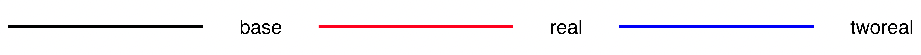
\includegraphics[width=0.5\textwidth]{Images/legend.png}
			\end{center}

			\begin{columns}
				\begin{column}{0.5\paperwidth}
					\begin{figure}
						\resizebox{\height}{4cm}{\includegraphics[width=0.9\paperwidth]{Images/popgrowth2.png}}
						\caption{Population growth}
					\end{figure}
				\end{column}

				\begin{column}{0.5\paperwidth}
					\begin{figure}
						\resizebox{\height}{4cm}{\includegraphics[width=0.9\paperwidth]{Images/popgrowth_diff.png}}
						\caption{\% Diff Population growth}
					\end{figure}
				\end{column}
			\end{columns}	

			\begin{itemize}
				\item Why? Differences in birth and death rates?
			\end{itemize}

		\end{frame}

		\begin{frame}{Birth Rate}
			\begin{center}
				\begin{figure}
					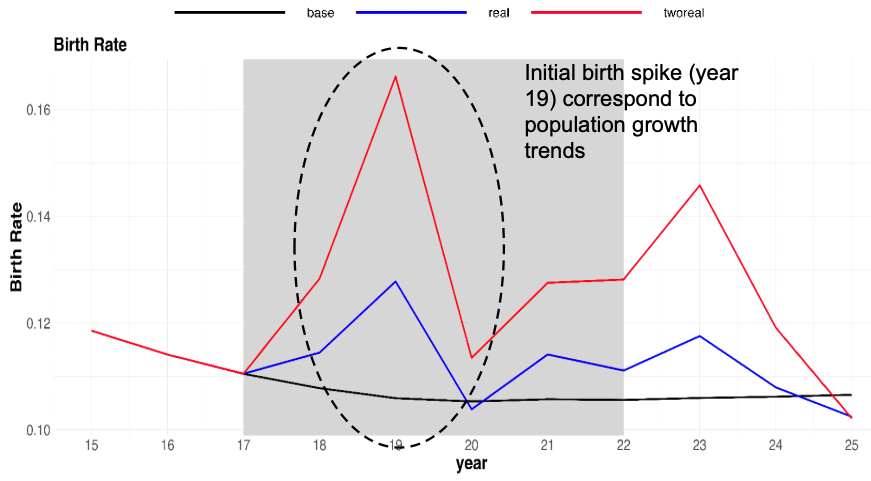
\includegraphics[width=\textwidth]{Images/birthrate.png}
					\caption{Birth rate (Conflict period)}
				\end{figure}
			\end{center} 	

			\begin{itemize}
				\item Shoter-term spikes in birth rates
			\end{itemize}

		\end{frame}

		\begin{frame}{Birth Rates}
			\begin{center}
				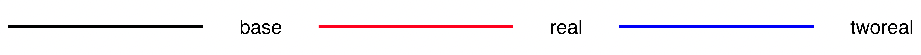
\includegraphics[width=0.5\textwidth]{Images/legend.png}
			\end{center}

			\begin{columns}
				\begin{column}{0.5\paperwidth}
					\begin{figure}
						\resizebox{\height}{4cm}{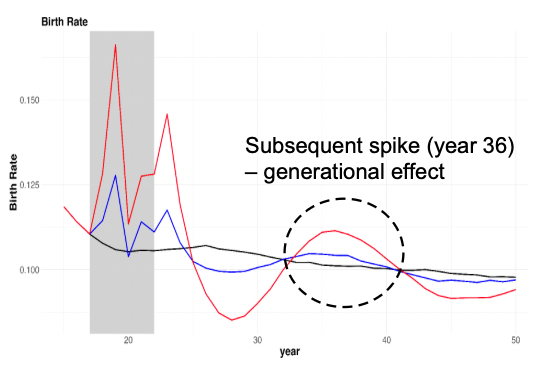
\includegraphics[width=0.7\paperwidth]{Images/birthrate2.png}}
						\caption{Birth Rates}
					\end{figure}
				\end{column}

				\begin{column}{0.5\paperwidth}
					\begin{figure}
						\resizebox{\height}{4cm}{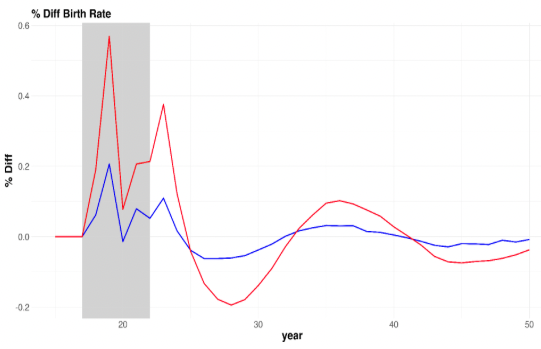
\includegraphics[width=0.7\paperwidth]{Images/birthrate_diff.png}}
						\caption{\% Diff Birth Rates}
					\end{figure}
				\end{column}
			\end{columns}	

			Short-term spikes in birth rates. Why?
			\begin{enumerate}
				\item Eligibility of birth (marriage)
				\item Behavioural equations (conflict events)
			\end{enumerate}
		\end{frame}

		\begin{frame}{Marriage Rates}
			\begin{center}
				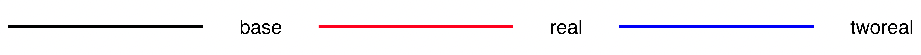
\includegraphics[width=0.5\textwidth]{Images/legend.png}
			\end{center}

			\begin{columns}
				\begin{column}{0.5\paperwidth}
					\begin{figure}
						\resizebox{\height}{4cm}{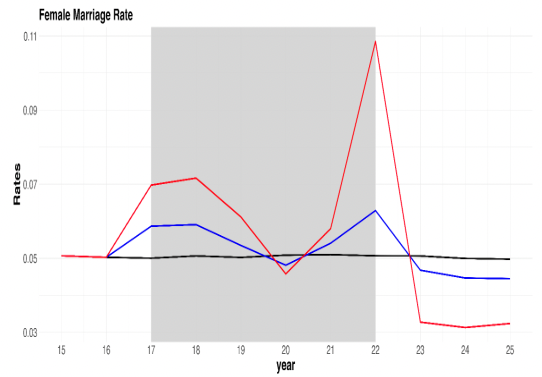
\includegraphics[width=0.7\paperwidth]{Images/marriage_female.png}}
						\caption{Female marriage rates (Conflict period)}
					\end{figure}
				\end{column}

				\begin{column}{0.5\paperwidth}
					\begin{figure}
						\resizebox{\height}{4cm}{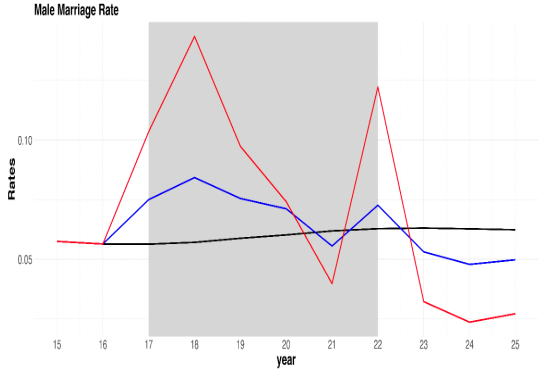
\includegraphics[width=0.7\paperwidth]{Images/marriage_male.png}}
						\caption{Male marriage rates (Conflict period)}
					\end{figure}
				\end{column}
			\end{columns}	

			\begin{itemize}
				\item Short-term spikes in marriage rates
			\end{itemize}
		\end{frame}

		\begin{frame}{Marriage Rates}
			\begin{center}
				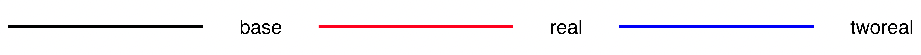
\includegraphics[width=0.5\textwidth]{Images/legend.png}
			\end{center}

			\begin{columns}
				\begin{column}{0.5\paperwidth}
					\begin{figure}
						\resizebox{\height}{4cm}{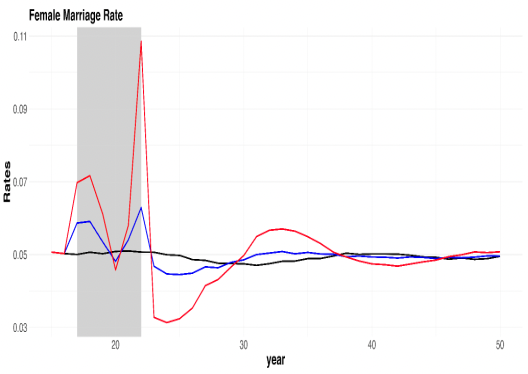
\includegraphics[width=0.6\paperwidth]{Images/marriage2_female.png}}
						\caption{Female marriage rates}
					\end{figure}
				\end{column}

				\begin{column}{0.5\paperwidth}
					\begin{figure}
						\resizebox{\height}{4cm}{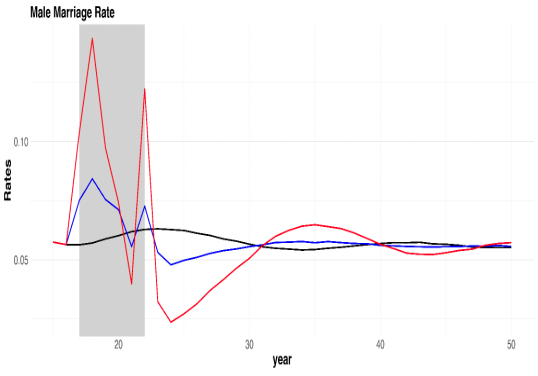
\includegraphics[width=0.6\paperwidth]{Images/marriage2_male.png}}
						\caption{Male marriage rates}
					\end{figure}
				\end{column}
			\end{columns}	

			\begin{itemize}
				\item Gender asymmetry in marriage proportions -- difference in behavioural equations?
				\item Effect on marriage weakens in the long term
			\end{itemize}
		\end{frame}

		\begin{frame}{Marriage and Birth Rates}
			\begin{center}
				
\includegraphics[width=0.5\textwidth]{Images/legend2.png}
			\end{center}

			\begin{columns}
				\begin{column}{0.5\paperwidth}
					\begin{figure}
						\resizebox{\height}{4cm}{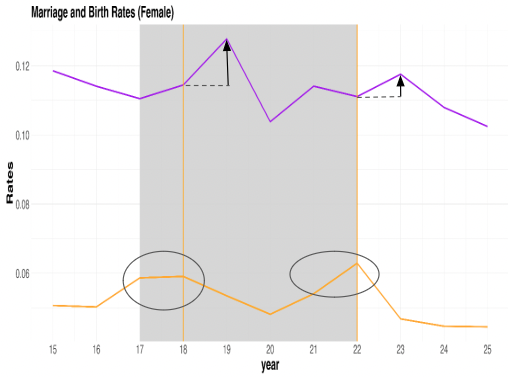
\includegraphics[width=0.6\paperwidth]{Images/marriage_birth_female.png}}
						\caption{Female marriage + birth rates}
					\end{figure}
				\end{column}

				\begin{column}{0.5\paperwidth}
					\begin{figure}
						\resizebox{\height}{4cm}{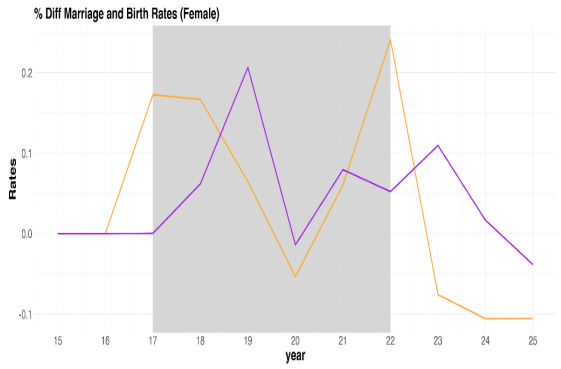
\includegraphics[width=0.6\paperwidth]{Images/marriage_birth_female2.png}}
						\caption{\% Diff Female marriage + birth rates}
					\end{figure}
				\end{column}
			\end{columns}	

			\begin{itemize}
				\item Peak in marriage rates precede peaks in birth rates \& population growth by 1 year
				\item Conflict events that affect birth rates too
			\end{itemize}
		\end{frame}

		\begin{frame}{Marriage and Birth Rates}
			\begin{center}
				
\includegraphics[width=0.5\textwidth]{Images/legend2.png}
			\end{center}

			\begin{columns}
				\begin{column}{0.5\paperwidth}
					\begin{figure}
						\resizebox{\height}{4cm}{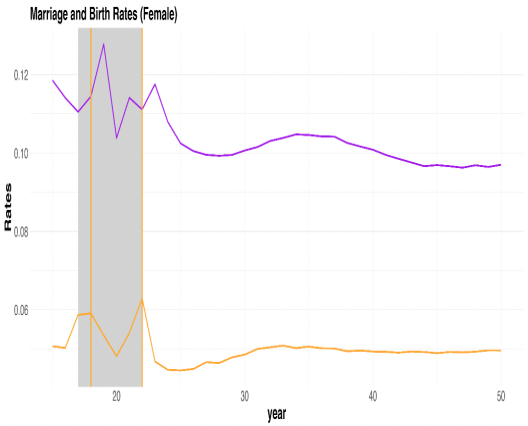
\includegraphics[width=0.6\paperwidth]{Images/marriage_birth_female3.png}}
						\caption{Female marriage + birth rates}
					\end{figure}
				\end{column}

				\begin{column}{0.5\paperwidth}
					\begin{figure}
						\resizebox{\height}{4cm}{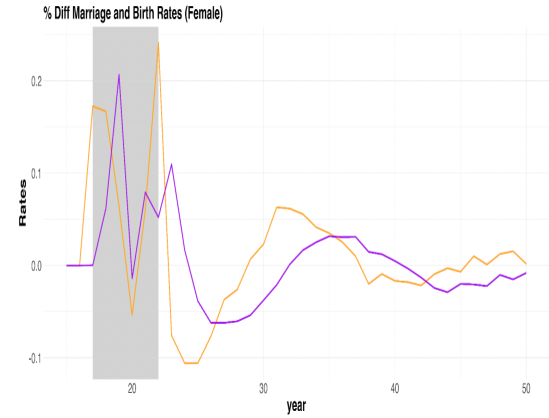
\includegraphics[width=0.6\paperwidth]{Images/marriage_birth_female4.png}}
						\caption{\% Diff Female marriage + birth rates}
					\end{figure}
				\end{column}
			\end{columns}	

			\begin{itemize}
				\item Trends in marriage rates precede birth rates
			\end{itemize}
		\end{frame}

\section{Conclusion}

	\begin{frame}{Conclusion}
		\textbf{Conflict increases population size}
		\begin{itemize}
			\item Short-term increases in marriage and birth
				\begin{itemize} 
					\item Long-term increase in population size
				\end{itemize}
			\item Long-term stability in population trajectories; but overall higher population size
		\end{itemize}
	\end{frame}
	
	\begin{frame}{Moving forward}
		\begin{itemize}
			\item Population age structure. Younger population? 
			\item Number of children ever born. Higher?
			\item Age at first marriage. Younger?
			\item Age at first birth
			\item Tempo of births
		\end{itemize}
	\end{frame}

\section{Questions}
	\begin{frame}{Questions}
		\begin{itemize}
			\item Birth Rate
				\begin{itemize}
					\item How do we distinguish between birth rate patterns due to marriage from other independent birth effects?
				\end{itemize}			
		\end{itemize}
	\end{frame}
\end{document}